% License: CC BY-SA
% Authors: See the authors below

\documentclass[25pt, margin=0mm, innermargin=25mm, blockverticalspace=25mm, colspace=25mm, subcolspace=8mm]{tikzposter}
\geometry{paperwidth=63in,paperheight=42in}

% to stretch boxes over whole paper with custor paper size
\makeatletter
\setlength{\TP@visibletextwidth}{\textwidth-2\TP@innermargin}
\setlength{\TP@visibletextheight}{\textheight-2\TP@innermargin}
\makeatother


\usepackage[utf8]{inputenc}
\usepackage{wrapfig}
\usepackage[hidelinks]{hyperref}

% For bibliography styling
%% TODO: all names should be abbreviated
\usepackage{natbib}

\renewcommand{\familydefault}{\sfdefault}

\definecolor{textcolor}{HTML}{000000}
\definecolor{viridisYellow}{HTML}{C1DF24}
\definecolor{viridisViolet}{HTML}{482173}
\definecolor{viridisGreen}{HTML}{51C46B}
\definecolor{viridisBlueGreen}{HTML}{209C8B}

\definecolorpalette{grassColorPalette} {
  \definecolor{colorOne}{HTML}{38588C}
  \definecolor{colorTwo}{HTML}{dddddd}
  \definecolor{colorThree}{named}{viridisYellow}
}

\usetheme{Default}
\usecolorstyle[colorPalette=grassColorPalette]{Britain}

\colorlet{backgroundcolor}{white}
\colorlet{framecolor}{viridisBlueGreen!90!white}
\colorlet{blocktitlebgcolor}{viridisBlueGreen!90!white}
\colorlet{blocktitlefgcolor}{white}

\title{
\fontsize{130}{100}\selectfont
Tools for Open Geospatial Science
}

% style for institute numbers
\newcommand{\inst}[1]{\hspace{2pt}$^{\mbox{\normalsize#1}}$\hspace{-7pt}}
\newcommand{\instlist}[1]{\hspace{1pt}$^{\mbox{\normalsize#1}}$\hspace{2pt}}

\author{
Vaclav Petras,
Anna Petrasova,
Helena Mitasova
}
\institute{
\large
North Carolina State University, Center for Geospatial Analytics, USA (wenzeslaus@gmail.com, vpetras@ncsu.edu)
\\[1.7cm]

\includegraphics{ncsu_cga}
}

\hypersetup
{
    pdfauthor={V. Petras, A. Petrasova, H. Mitasova},
    pdfsubject={Challenges and Benefits of Open Source Software and Open Data},
    pdftitle={Tools for open geospatial science},
    pdfkeywords={open science, reproducibility, replicability, GIS, geospatial, open source, FOSS, FLOSS, methods, preservation}
}

% directories with images in the course
\graphicspath{{img/}{img/logos/}{../img/}{../lectures/img/}{../lectures/img/logos/}}

\newcommand{\blocktitlewrap}[1]{\textsf{\textbf{\Huge#1}}}
% it is not possible (?) to change block title in the class, using wrapper
% the command introduced using:
%   sed -i 's/\\block{\([^}]*\)}/\\block{\\blocktitlewrap{\1}}/g' main.tex


%%%%%%%%%%%%%%%%%%%%%%%%%%%%%%%%%%%%%%%%%%%%%%%%%%%%%%%%%%%%%%%%%%%%%
%%%%%%%%%%%%%%%%%%%%%%%%%%%%%%%%%%%%%%%%%%%%%%%%%%%%%%%%%%%%%%%%%%%%%
%%%%%%%%%%%%%%%%%%%%%%%%%%%%%%%%%%%%%%%%%%%%%%%%%%%%%%%%%%%%%%%%%%%%%
%%%%%%%%%%%%%%%%%%%%%%%%%%%%%%%%%%%%%%%%%%%%%%%%%%%%%%%%%%%%%%%%%%%%%
\begin{document}

\node[below left,opacity=0.93,inner sep=0pt,outer sep=0pt] at (topright)%
  {
\includegraphics[trim={0 0 0 8cm},clip,width=\paperwidth]{viridis_wheels}};

\node[above right,opacity=0.99,inner sep=0pt,outer sep=0pt] at (bottomleft)%
  {
\includegraphics[trim={0 8cm 0 0},clip,width=\paperwidth]{viridis_wheels}};

\maketitle[width=0.5\textwidth,linewidth=1cm,innersep=2cm]

\begin{columns}

%%%%%%%%%%%%%%%%%%%%%%%%%%%%%%%%%%%%%%%%%%%%%%%%%%%%%%%%%%%%%%%%%%%%%
%%%%%%%%%%%%%%%%%%%%%%%%%%%%%%%%%%%%%%%%%%%%%%%%%%%%%%%%%%%%%%%%%%%%%
%%%%%%%%%%%%%%%%%%%%%%%%%%%%%%%%%%%%%%%%%%%%%%%%%%%%%%%%%%%%%%%%%%%%%
%%%%%%%%%%%%%%%%%%%%%%%%%%%%%%%%%%%%%%%%%%%%%%%%%%%%%%%%%%%%%%%%%%%%%
\column{0.25}

%%%%%%%%%%%%%%%%%%%%%%%%%%%%%%%%%%%%%%%%%%%%%%%%%%%%%%%%%%%%%%%%%%%%%%%%%%%%%%%%
\block{\blocktitlewrap{Highlights}}
{

\LARGE

% \setlength{\parskip}{0.3ex}

\renewcommand{\labelitemi}{\textcolor{gray}{$\bullet$}\hspace{0.5ex}}
\newcommand{\blocksectiontitle}[1]{\bigskip\textbf{\textcolor{gray}{\textsf{#1}}}}

% Open science uses open source to deal with reproducibility challenges in data and computational sciences. However, just using open source software or making the code public does not make the research reproducible. Moreover, the scientists face the challenge of learning new unfamiliar tools and workflows. In this contribution, we will look at a graduate-level course syllabus covering several software tools which make validation and reuse by a wider professional community possible. For the novices in the open science arena, we will look at how scripting languages such as Python and Bash help us reproduce research (starting with our own work). Jupyter Notebook will be introduced as a code editor, data exploration tool, and a lab notebook. We will see how Git helps us not to get lost in revisions and how Docker is used to wrap all the parts together using a single text file so that figures for a scientific paper or a technical report can be generated with a single command. We will look at examples of software and publications in the geospatial domain which use these tools and principles. Scientific contributions to GRASS GIS, a powerful open source desktop GIS and geoprocessing backend, will serve as an example of why and how to publish new algorithms and tools as part of a bigger open source project.

% Open science uses open source to deal with reproducibility in data and computational sciences, but just using open source or making the code public does not make the research reproducible. In this contribution, we present a syllabus for open science graduate-level course. The course covers several software tools and workflows which make validation and reuse of research possible and much easier. The course further covers scripting and automation, interactive notebooks, tracking of changes, and sharing research in a way. The course shows examples of software and publications in the geospatial domain which use these tools and principles. This contribution will specifically show scientific contributions to GRASS GIS, a powerful open source desktop GIS and geoprocessing backend, as a use case of publishing new algorithms in a large and established open source project.

\blocksectiontitle{Course highlights}

\begin{itemize}
 \item Complete graduate-level course with all material available.
 \item Course taught at NCSU CGA, for 15 on-campus and off-campus students, fall semester 2017.
\end{itemize}

\blocksectiontitle{Motivation}

\begin{itemize}
 \item \textit{It's impossible to conduct research without software...}
  \citep{hettrick2014uk, hettrick2014impossible}
 % cite: Hettrick et al, UK Research Software Survey 2014
 \item \textit{Software [...] developed as part of novel methods is as important for the method's implementation [...] Such software [...] must be made available to readers upon publication.}
  \citep{socialsoftware2007}.
 % cite: Nature Methods - 4, 189 (2007) doi:10.1038/nmeth0307-189
%  \item Paper is not enough to register, archive, disseminate and peer review.
 \item Various authors over the last 20 years identified
that text is less than sufficient way of communicating research and described reproducibility spectrum
\citep{buckheit1995wavelab, peng2011reproducible, rodriguez2016ciencia, marwick2017computational}.
\end{itemize}

}

% %%%%%%%%%%%%%%%%%%%%%%%%%%%%%%%%%%%%%%%%%%%%%%%%%%%%%%%%%%%%%%%%%%%%%%%%%%%%%%%
% \block{\blocktitlewrap{Reproducibility Spectrum}}{
%
% Various authors over the last 20 years identified
% that text is less than sufficient way of communicating research
% \citep{buckheit1995wavelab, peng2011reproducible, rodriguez2016ciencia, marwick2017computational}.
%
% \vspace{1ex}
%
% \centering
% 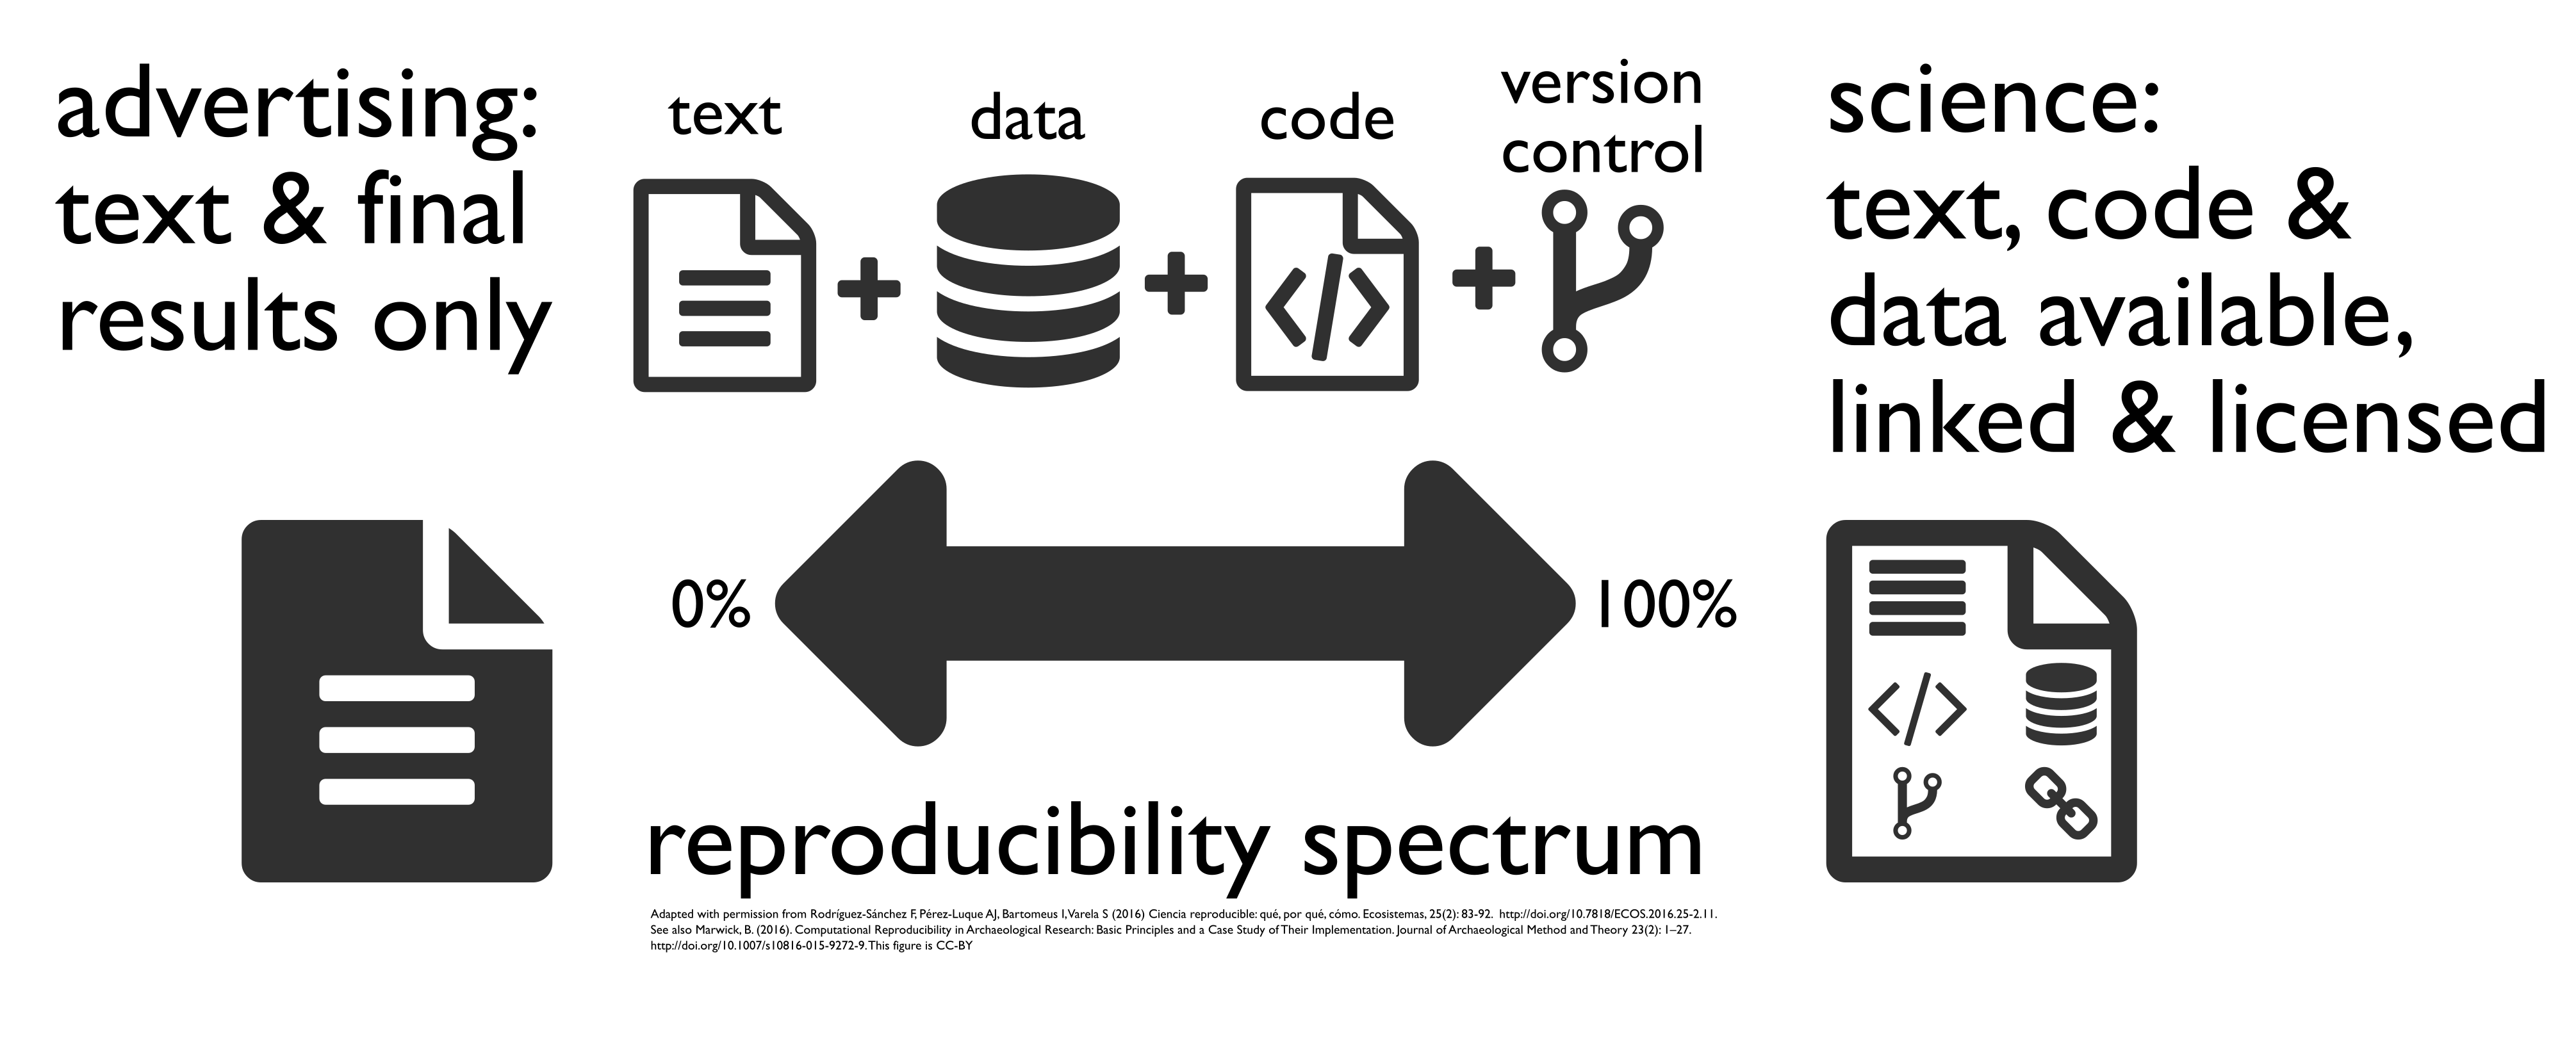
\includegraphics[width=\linewidth]{spectrum_of_reproducible_research}
% \scriptsize
% \vspace{1ex}
% Image credit: CC BY-SA Comtebenoit, Wikimedia
%
% \vspace{-7mm}
%
% }

%%%%%%%%%%%%%%%%%%%%%%%%%%%%%%%%%%%%%%%%%%%%%%%%%%%%%%%%%%%%%%%%%%%%%%%%%%%%%%%
\block{\blocktitlewrap{Course Syllabus}}{

\Large

\renewcommand{\labelitemi}{\textcolor{gray}{$\bullet$}\hspace{0.5ex}}

\begin{itemize}
% Basic Topics
 \item Introduction to and motivation for open science
 \item Collaborative writing of scientific papers (Authorea, Markdown)
 \item Advanced tools for papers and reports (Overleaf, LaTeX)
 \item Revision control systems and wiki technologies (Git, GitHub)
 \item How open source communities and development work
% Geospatial Topics
 \item QGIS, a free and open source geographic system
 \item Command line and remote access to computational resources
 \item Command line and Python tools for geospatial work (GDAL)
 \item GRASS GIS as software for geospatial research
 \item Publishing data on web (data repositories, OpenLayers)
%  Advanced Topics
 \item Combining text, code and results into one document (Jupyter)
 \item Publishing code as part of an open source project
 \item Reproducible computational environments (Docker)
 \item Writing and reproducing an open science paper
\end{itemize}

}

% %%%%%%%%%%%%%%%%%%%%%%%%%%%%%%%%%%%%%%%%%%%%%%%%%%%%%%%%%%%%%%%%%%%%%%%%%%%%%%%
% \block{\blocktitlewrap{Research publication components}}{
%
% \begin{center}
% 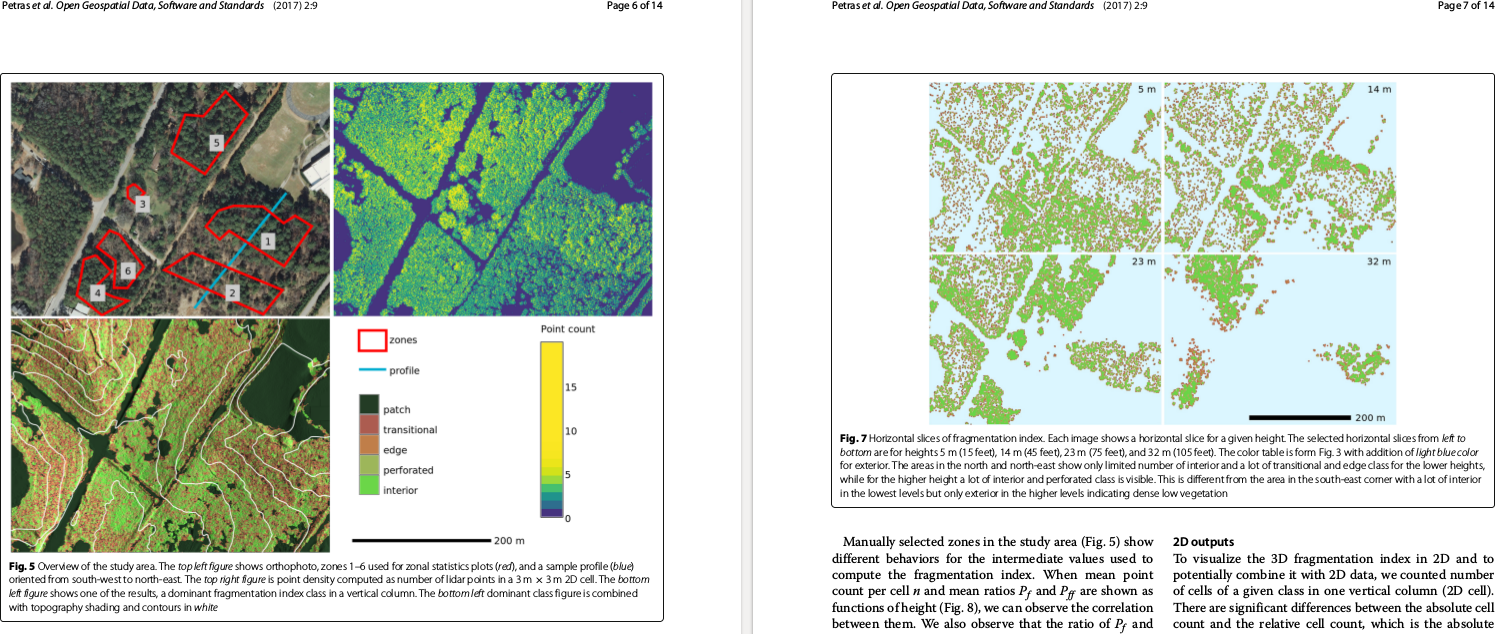
\includegraphics[width=\linewidth]{petras2017generalized_paper_detail}
% \end{center}
%
% \begin{tabular}{lll}
% \textbf{Component} & \textbf{Content} & \textbf{Technology} \\
% % \hline
% Text & background, methods, results, discussion & PDF, HTML, * \\
% Data & collected data and computational results & open formats, ** \\
% Reusable code & generally and reusably implemented methods & Python, R, C \\
% Specific code & scripts to generate results & Bash, Python, R, ** \\
% Environment & details about all dependencies and the code & Docker, Vagrant \\
% Versions & repository with current and previous versions & Git, Mercurial \\
% \end{tabular}
%
% {
% * Source format being e.g. LaTeX or Markdown\\
% ** Potentially included in computational notebooks such as Jupyter Notebook
% }
%
% Example (paper):
% Petras, V., Newcomb, D. J., \& Mitasova, H. (2017).
% Generalized 3D fragmentation index derived from lidar point clouds.
% \textit{Open Geospatial Data, Software and Standards},
% 2(1), 9. doi:10.1186/s40965-017-0021-8
%
% }

%%%%%%%%%%%%%%%%%%%%%%%%%%%%%%%%%%%%%%%%%%%%%%%%%%%%%%%%%%%%%%%%%%%%%
%%%%%%%%%%%%%%%%%%%%%%%%%%%%%%%%%%%%%%%%%%%%%%%%%%%%%%%%%%%%%%%%%%%%%
%%%%%%%%%%%%%%%%%%%%%%%%%%%%%%%%%%%%%%%%%%%%%%%%%%%%%%%%%%%%%%%%%%%%%
%%%%%%%%%%%%%%%%%%%%%%%%%%%%%%%%%%%%%%%%%%%%%%%%%%%%%%%%%%%%%%%%%%%%%
\column{0.25}


%%%%%%%%%%%%%%%%%%%%%%%%%%%%%%%%%%%%%%%%%%%%%%%%%%%%%%%%%%%%%%%%%%%%%%%%%%%%%%%
\block{\blocktitlewrap{Scripting}}{

\LARGE

Automation in lab work, repeatability by others, and review by peers is enabled by scripting.
However, the natural way to capture workflows in graphical user interface is
taking screenshots such as this series from GRASS GIS:

\begin{center}
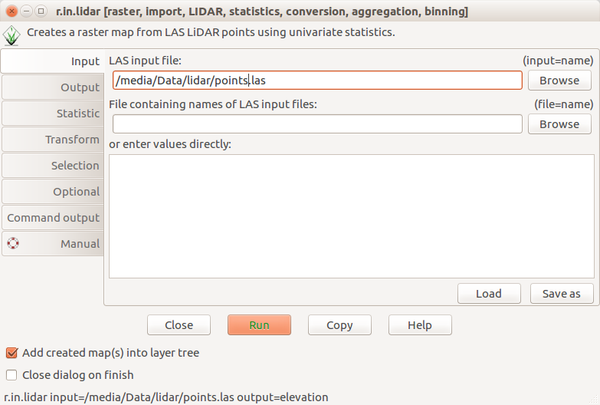
\includegraphics[width=0.3\linewidth]{r_in_lidar_1}
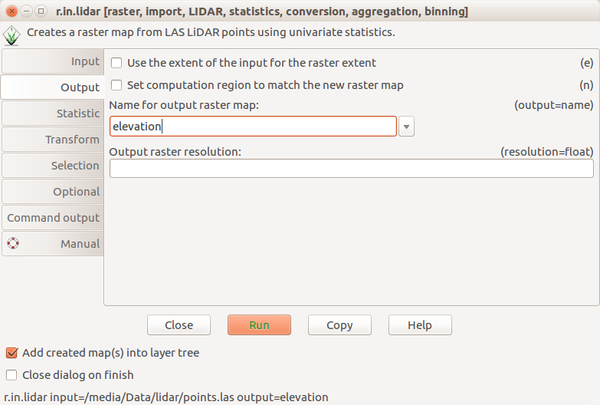
\includegraphics[width=0.3\linewidth]{r_in_lidar_2}
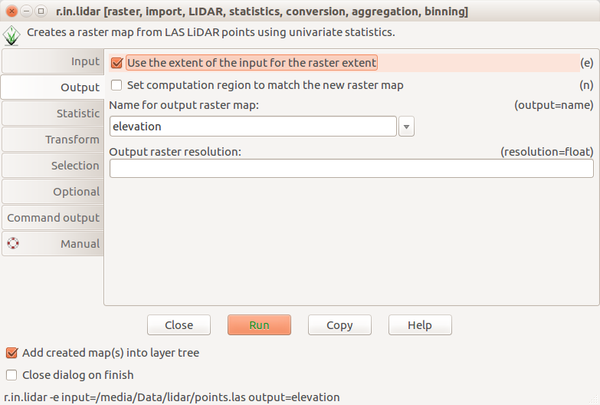
\includegraphics[width=0.3\linewidth]{r_in_lidar_3}
\end{center}

Scripting is a more efficient way of recording the same information
which can be edited and automatically processed.
The following Bash command is equivalent of the three screenshots above:

\Large

\begin{center}
% Bash and GRASS GIS:\\
\texttt{r.in.lidar input=points.las output=elevation -e}\\
% Python and GRASS GIS:\\
% \texttt{run\_command("r.in.lidar", input="points.las", output="elevation", flags="e")}\\
% R and GRASS GIS:\\
% \texttt{execGRASS("r.in.lidar", input="points.las", output="elevation", flags="e")}\\
\end{center}

\normalsize

Languages used in the class: Python and Bash;
Alternatives: R, Ruby, Octave, Julia, ...

}

%%%%%%%%%%%%%%%%%%%%%%%%%%%%%%%%%%%%%%%%%%%%%%%%%%%%%%%%%%%%%%%%%%%%%%%%%%%%%%%
\block{\blocktitlewrap{Versioning \& Publishing Code}}{
% \block{\blocktitlewrap{Revision control}}{

\LARGE

File format and software-dependent concepts of file versioning are
replaced by scalable and robust techniques.

\vspace*{0.7cm}

\begin{center}
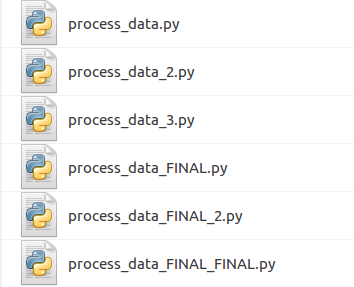
\includegraphics[width=0.25\linewidth]{file_versions}
\begin{minipage}{0.05\linewidth}
{\Huge $\rightarrow$}
{
\normalsize
\rule{0pt}{12ex}
}
\end{minipage}
\begin{minipage}[b]{0.45\linewidth}
\centering
{
\normalsize
\texttt{git commit process\_data.py -m "replaced part of the main equation"}\\
}
\vspace*{1ex}
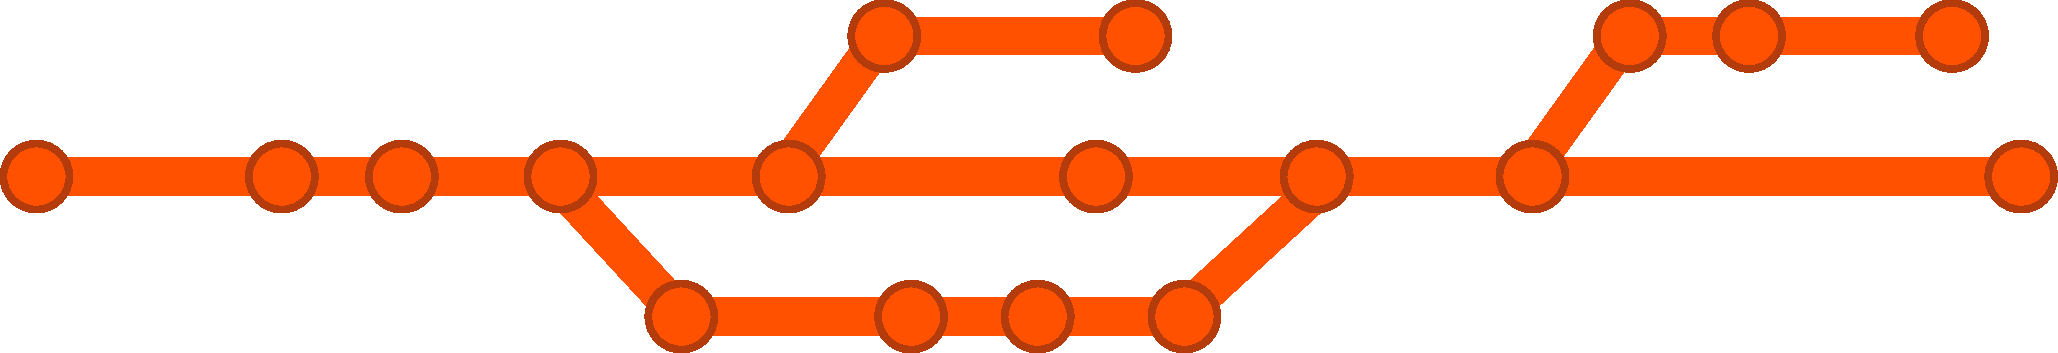
\includegraphics[width=\linewidth]{revisions}
\end{minipage}
\end{center}

\normalsize

\vspace*{-4ex}

Software used in class: Git (\texttt{git}).
% \\
Alternatives: Subversion (\texttt{svn}), Mercurial (\texttt{hg}), ...

Hosting option used in class: GitHub.
% \\
Self-hosted open alternatives: GitLab, Gogs, Gitolite, Trac, ...
% \\
Alternative services: GitLab, Bitbucket, ...

% }

%%%%%%%%%%%%%%%%%%%%%%%%%%%%%%%%%%%%%%%%%%%%%%%%%%%%%%%%%%%%%%%%%%%%%%%%%%%%%%%
% \block{\blocktitlewrap{Publishing Code}}{

\LARGE

Publishing code can be as simple as uploading file online using a web browser,
however more advanced ways such as integration into a larger open source project
bring many benefits.

\normalsize

Why?
Preprocessing, visualization, and user interface (GUI, CLI, API),
inputs, outputs, memory management and other common features,
integration with existing analytical tools,
long-term maintenance.
Options: R package, Python package, GRASS GIS module, QGIS plugin, ...
Integration gradient: unofficial extension - integrated extension - code addition.
Licensing and criteria to choosing the project \citep{schweik2012internet}
need to be part of the course.

\begin{center}

\includegraphics[height=.11\linewidth]{octocat}
~

\includegraphics[height=.11\linewidth]{grass}
~

\includegraphics[height=.11\linewidth]{gpl}
\end{center}

}


%%%%%%%%%%%%%%%%%%%%%%%%%%%%%%%%%%%%%%%%%%%%%%%%%%%%%%%%%%%%%%%%%%%%
%%%%%%%%%%%%%%%%%%%%%%%%%%%%%%%%%%%%%%%%%%%%%%%%%%%%%%%%%%%%%%%%%%%%%
\column{0.25}

%%%%%%%%%%%%%%%%%%%%%%%%%%%%%%%%%%%%%%%%%%%%%%%%%%%%%%%%%%%%%%%%%%%%%%%%%%%%%%%
\block{\blocktitlewrap{Computational Notebooks}}{

\LARGE

Computational notebooks are interactive documents with text, code, and figures.
Notebooks work for most languages and can be exported to many formats
for publication online or print. Content can range from class assignments to full
papers or interactive figures in published papers.

\vspace*{0.7cm}

\begin{center}
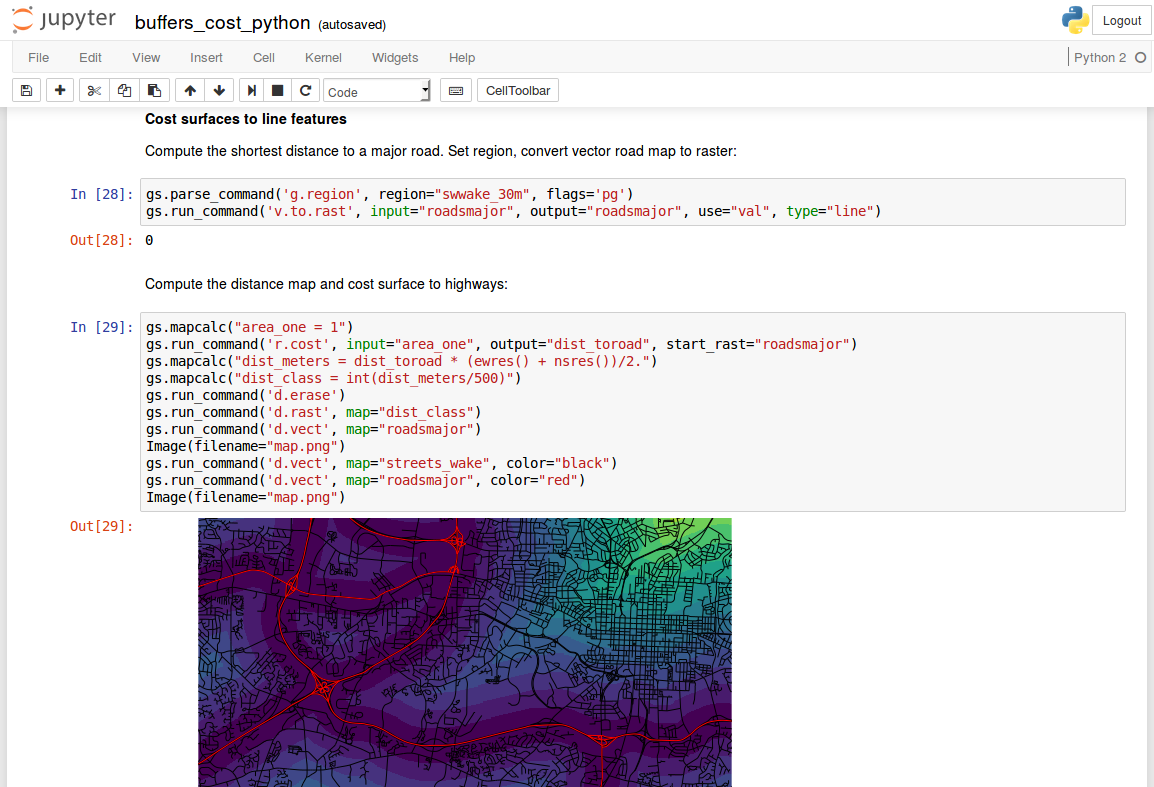
\includegraphics[width=\linewidth]{jupyter}
\end{center}

\normalsize

Used in the class: Jupyter Notebook;
Alternatives: R Markdown (Notebook), Emacs Org-mode, ...

}


%%%%%%%%%%%%%%%%%%%%%%%%%%%%%%%%%%%%%%%%%%%%%%%%%%%%%%%%%%%%%%%%%%%%%%%%%%%%%%%
\block{\blocktitlewrap{Runtime Environments}}{

\LARGE

To run any code, various dependencies need to be available,
which is often challenging.
% description, completeness and availability.
Solutions include Docker, Vagrant, and virtual machines
which create full and self-contained environments.
The following is a example of environment description for Docker:

\vspace*{0.7cm}

\begin{center}
\begin{minipage}{0.9\linewidth}
\begin{flushleft}
\tt
\textit{\# Dockerfile}\\
FROM ubuntu:16.04\\
RUN apt-get update\\
RUN apt-get install -y python sqlite3\\
WORKDIR /data\\
\end{flushleft}
\end{minipage}
\end{center}

\begin{center}

\includegraphics[trim={0 0 10cm 0}, clip, width=0.22\linewidth]{docker}
\end{center}

}


%%%%%%%%%%%%%%%%%%%%%%%%%%%%%%%%%%%%%%%%%%%%%%%%%%%%%%%%%%%%%%%%%%%%%
%%%%%%%%%%%%%%%%%%%%%%%%%%%%%%%%%%%%%%%%%%%%%%%%%%%%%%%%%%%%%%%%%%%%%
%%%%%%%%%%%%%%%%%%%%%%%%%%%%%%%%%%%%%%%%%%%%%%%%%%%%%%%%%%%%%%%%%%%%%
%%%%%%%%%%%%%%%%%%%%%%%%%%%%%%%%%%%%%%%%%%%%%%%%%%%%%%%%%%%%%%%%%%%%%
\column{0.25}

%%%%%%%%%%%%%%%%%%%%%%%%%%%%%%%%%%%%%%%%%%%%%%%%%%%%%%%%%%%%%%%%%%%%%%%%%%%%%%%
\block{\blocktitlewrap{Examples of Research}}{

\LARGE

\newcommand{\blocksectiontitle}[1]{\bigskip\textbf{\textcolor{gray}{\textsf{#1}}}}

\blocksectiontitle{Lidar Analysis}

Lidar analysis paper by \cite{petras2017generalized} is an example of
research which provided scripts needed to produce figures presented in the paper
as well as reusable code which was published as a module in GRASS GIS Addons repository.

\vspace*{0.7cm}

\begin{center}
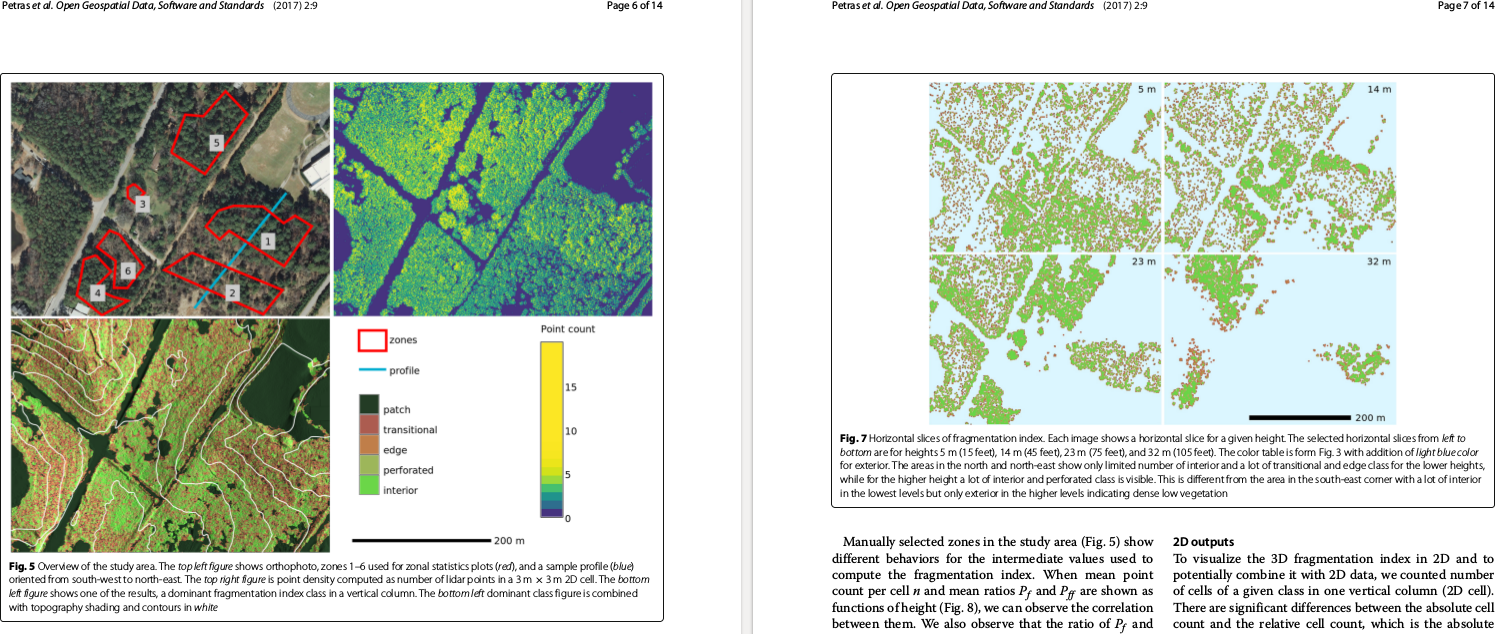
\includegraphics[width=\linewidth]{petras2017generalized_paper_detail}
\end{center}

\blocksectiontitle{Urbanization}

Landscape change and urbanization paper by \cite{petrasova2016open} is an example
of research which turned unpublished code into reusable tool for modeling
available as a set of modules in GRASS GIS Addons repository.

\vspace*{0.7cm}

\begin{center}
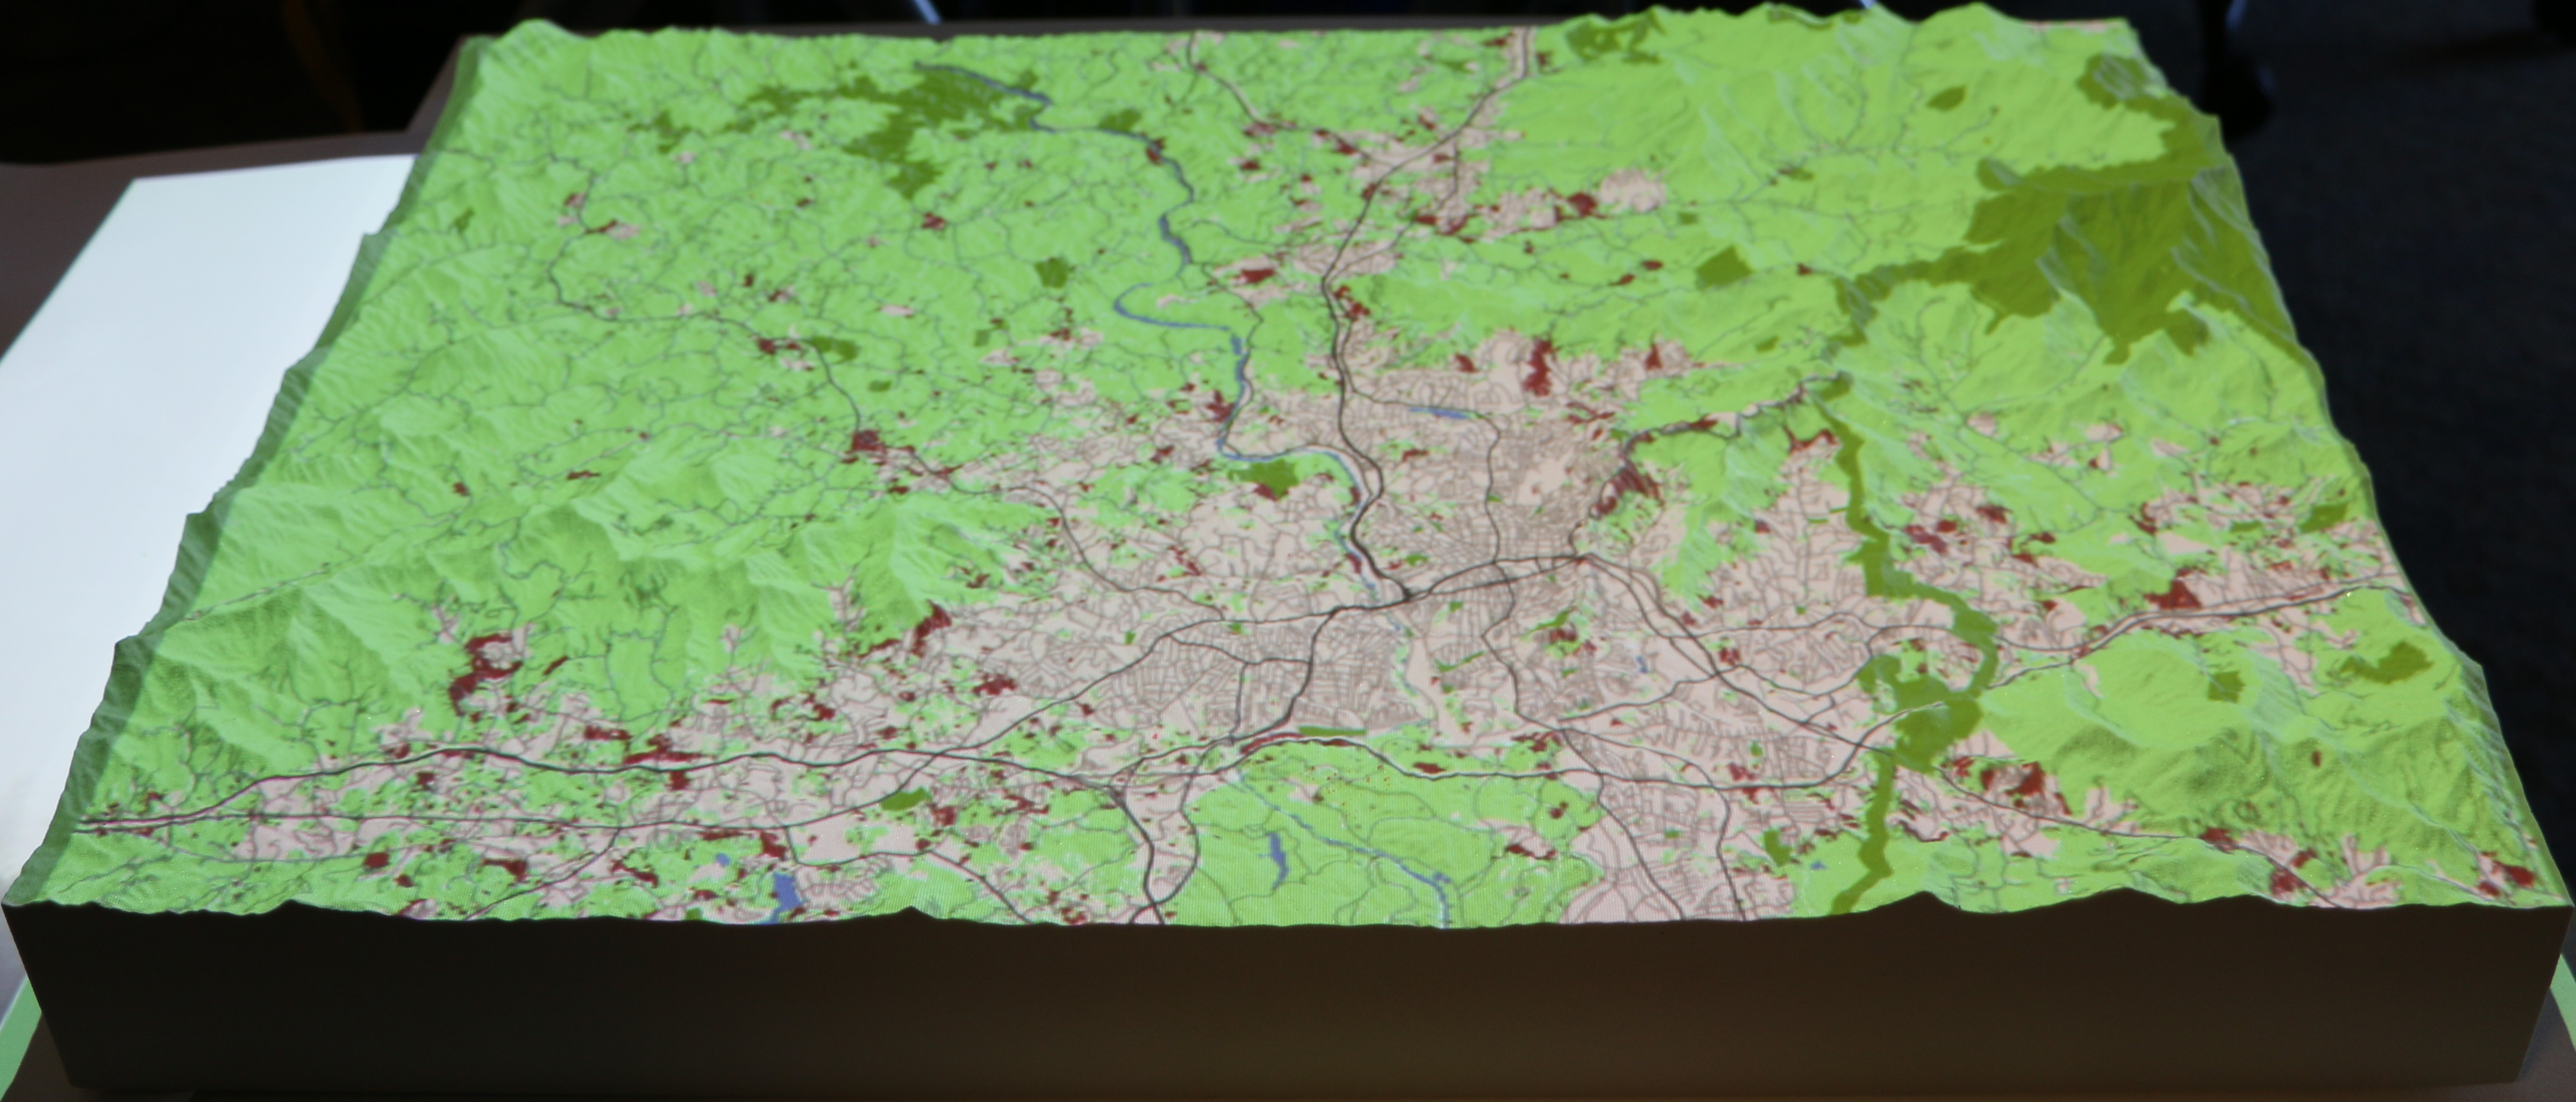
\includegraphics[width=\linewidth]{futures}
\end{center}

}

%%%%%%%%%%%%%%%%%%%%%%%%%%%%%%%%%%%%%%%%%%%%%%%%%%%%%%%%%%%%%%%%%%%%%%%%%%%%%%%%
\block{\blocktitlewrap{References \& Resources}}{

\vspace{-0.2cm}
\scriptsize

% \newcommand{\blocksectiontitle}[1]{\subsubsection*{\textcolor{gray}{\textsf{#1}}}}
\newcommand{\blocksectiontitle}[1]{\textbf{#1}}

%\blocksectiontitle{References}
\begingroup
\renewcommand{\section}[2]{}%
\bibliographystyle{apalike}
\bibliography{poster}
\endgroup


\vspace{0.2cm}

\textcolor{gray}{
\hrulefill
}

\vspace{0.1cm}

\newcommand{\qrcodesize}{0.05\linewidth}

% qrencode http://grass.osgeo.org -o qr_grass.eps -t EPS
% epspdf -b qr_grass.eps qr_grass.pdf

\begin{center}
\begin{tabular}{c}

\begin{minipage}{\qrcodesize}

\includegraphics[width=\textwidth]{url_g8pFiE_qrcode.png}
\end{minipage}
~
\begin{minipage}{0.15\linewidth}
\small {\href{https://goo.gl/g8pFiE}{\nolinkurl{goo.gl/g8pFiE}}}
\end{minipage}
\hspace{0.1\linewidth}
\begin{minipage}{0.1\linewidth}
\href{http://creativecommons.org/licenses/by-sa/4.0/}{
\includegraphics[width=\textwidth]{ccbysa}}
\end{minipage}
~
\begin{minipage}{0.35\linewidth}
\small This poster is licensed under a Creative Commons Attribution-ShareAlike 4.0 International License.
\end{minipage}

\end{tabular}
\end{center}

Course material is available at the above address and the formats and software used for publishing
is described in \cite{petras2015integrating}.

\vspace{-0.08cm}

}

\end{columns}

\node[above right,opacity=0.07,inner sep=0pt,outer sep=0pt] at (bottomleft)%
  {
\includegraphics[trim={0 8cm 0 0},clip,width=\paperwidth]{viridis_wheels}};

\end{document}
